\documentclass[12pt]{book}
\usepackage{booktabs}
\usepackage[table]{xcolor}
\usepackage{tcolorbox}
\usepackage[T1]{fontenc}
\usepackage{wrapfig}
\usepackage{url}
\usepackage{dsfont}
\usepackage{enumitem}
\usepackage{array}
\usepackage{booktabs}
\usepackage{multirow}
\usepackage{mathtools, nccmath}
\usepackage[polish]{babel}
\usepackage[utf8]{inputenc}
\usepackage{empheq}
\usepackage{lmodern}
\usepackage{cleveref}
\usepackage{pifont}
\usepackage{blkarray, bigstrut}
\usepackage{amsmath}
\usepackage{kbordermatrix}
\usepackage{bbm}
\usepackage{dsfont}
\usepackage{cases}
\usepackage{graphicx}
\usepackage{cellspace}
\usepackage[T1]{fontenc}
\usepackage{amsthm}
\selectlanguage{polish}
\usepackage{amsmath}
\usepackage{graphicx}
\usepackage{float}
\usepackage{cite}
\usepackage[margin=2.5cm]{geometry}
\theoremstyle{plain}
\newtheorem{definicja}{Definicja}
\newtheorem{twr}{Twierdzenie}
\newtheorem{lem}[twr]{Lemat}
\newtheorem{mur}{Murphy}[section]
\newcolumntype{P}[1]{>{\centering\arraybackslash}p{#1}}
\newcommand\green{\cellcolor{green!10}}
\newcommand\cincludegraphics[2][]{\raisebox{-0.5\height}{\includegraphics[#1]{#2}}}
\newcommand\red{\cellcolor{red!20}}
\newcommand\blue{\cellcolor{blue!20}}
\newcommand{\R}{\mathbb{R}}
\newcommand*{\tabbox}[2][t]{%
	\vspace{0pt}\parbox[#1][3.7\baselineskip]{1cm}{\strut#2\strut}}
\newcommand\addtag{\refstepcounter{equation}
	\renewcommand{\labelenumii}{\theenumii}
	\renewcommand{\theenumii}{\theenumi.\arabic{enumii}.}
	\tag{\theequation}}
\newcommand{\specialcell}[2][c]{%
	\begin{tabular}[#1]{@{}c@{}}#2\end{tabular}}
\let\oldref\ref
\renewcommand{\ref}[1]{(\oldref{#1})}

\begin{document}
	\title{Optymalizacja  systemu sygnalizacji świetlnej w 
		oparciu o przepływowy model ruchu pojazdów.}
	\author{Michał Lis}
	\date{\today}
	\maketitle
	\tableofcontents
	
	\chapter {Środowiska symulacyjne i ich nauka}
	\section{Środowisko 11}
	\begin{figure}[H]
		\centering
		
\includegraphics[width=10cm]{images/env_11}
		\label{fig:env_11}
		\caption{środowisko 11}
	\end{figure}
	
	Środowisko posiada 3 jednokierunkowe drogi. Każda droga ma 2 odcinki co daje w sumie 6 odcinków (są numerowane od 0 co widać na rysunku \ref{fig:env_11}).
	W sieci dróg znajduje się jedno skrzyżowanie. Jest do niego przypisany agent, który odpowiada za sterowanie sygnalizacją świetlną.
	
\subsection{Sygnalizacje świetlne}	
	\begin{figure}[H]
		\centering
		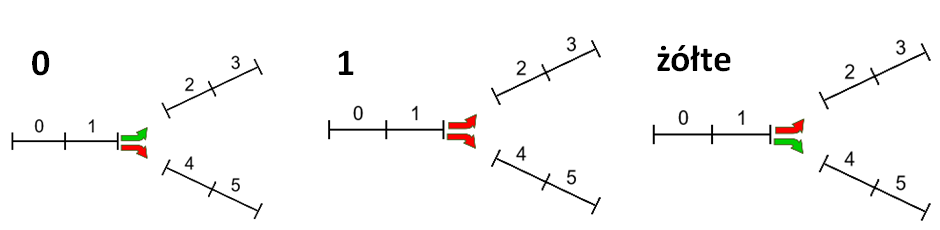
\includegraphics[width=17cm]{images/env_11_fazy}
		\label{fig:env_11_fazy}
		\caption{środowisko 11 - fazy świateł}
	\end{figure}\noindent
Skrzyżowanie posiada 3 fazy świetlne przedstawione powyżej. Fazy 0 i 1 posiadają pewne zielone światła i umożliwiają ruch. Automatycznie ustawiana jest faza żółtych świateł przez 2 interwały czasowe w przypadku podjęcia akcji zmiany aktualnej fazy. Agent może także oczywiście przedłużyć aktualną fazę.
\subsection{Możliwe do wykonania manewry}
Niech wektor $ [i,j] $ będzie manewrem polegającym na bezpośrednim przejeździe z odcinka $ i $ na odcinek $ j $. Zostanie teraz zdefiniowana macierz sygnalizacji świetlnej $\textbf{S}$. Określa ona wykonalność dowolnego manewru.
\begin{numcases}{S_{ij}=}
0 & dla niemożliwego manewru \label{eq:manewr_not_existing} \\
0 & dla manewru wstrzymanego przez czerwone światło \label{eq:stopped_by_light} \\
1 & dla manewru zezwolonego przez zielone światło \label{eq:allowed_by_light} \\
1 & dla manewru nie wymagającego sygnalizacji świetlnej \label{eq:manewr_existing}
\end{numcases}
Przykłady poszczególnych manewrów są następujące:
\begin{itemize}
\item \ref{eq:manewr_not_existing} Niemożliwym manewrem jest np. $ [0,2] $, gdyż nie ma możliwości bezpośredniego przejazdu z odcinka $ 0 $ do $ 2 $.
\item \ref{eq:stopped_by_light} - Dla fazy świetlnej $ 0 $ manewrem zatrzymanym przez czerwone światło  jest $ [1,4] $.
\item \ref{eq:allowed_by_light} - Manewrem zezwolonym przez zielone światło  dla fazy $ 0 $ jest $ [1,2] $.
\item \ref{eq:manewr_existing} - Prawidłowym manewrem bez sygnalizacji świetlnej są manewry $ [0,1] $, $ [2,3] $, $ [4,5] $.
\end{itemize}

\subsection{Przepływ pojazdów}

\begin{figure}[H]
	\centering
	\includegraphics[width=10cm]{images/env_11_RUCH}
	\label{fig:env_11_RUCH}
	\caption{środowisko 11 - fazy świateł}
\end{figure}\noindent
Pojazdy pokonują jeden odcinek podczas jednego pełnego interwału czasowego. Skrzyżowanie posiada dwa możliwe manewry do wykonania. Dla każdego pojazdu prawdopodobieństwo skrętu w prawo to 70 procent. Jazda w lewo z kolei to pozostałe 30 procent prawdopodobieństwa. Taki sposób przepływu definiuje rzadką macierz prawdopodobieństwa $ \textbf{P} $ o wymiarach 6 na 6. 
\begin{itemize}
	\item $\textbf{P}[1,2]=0.3$ wyznacza manewr skrętu w lewo
	\item $\textbf{P}[1,4]=0.7$ wyznacza manewr skrętu w prawo
	\item $\textbf{P}[0,1]=1 \;\; \textbf{P}[2,3]=1 \;\; \textbf{P}[4,5]=1$ co wynika z przepływu pojazdów pomiędzy sekcjami na jednej drodze
	\item Pozostałe wartości macierzy $\textbf{P}$ to zera
\end{itemize}

\clearpage \noindent
%Odpływ pojazdów z układu następuje na końcach odcinków 29,32 oraz 35. Z tego względu zostaje wprowadzona macierz rzadka $\mathbbm{1}$ o wymiarach 36 na 36. Ma ona na celu usuwać pojazdy opuszczające układ.
%\begin{numcases}{\mathbbm{1}_{mn}=}
%0 & dla $m \neq n \vee n \in {29,32,35}$ \\
%1 & dla pozostałych przypadków
%\end{numcases}
%Wiersze i kolumny macierzy są numerowane od 0 - zgodnie z konwencją przyjętą w pracy.
Macierz stanowa A jest określona następująco:
\begin{numcases}{A_{ij}=}
0 & dla $S[i,j]=0 \vee i \in {3,5}$ \\
P[i,j] & dla $ S[i,j]=1$ \\
1-\delta(i) & dla $i=j \wedge  i \not\in {3,5}$
\end{numcases}
Gdzie delta jest sumą wszystkich pozostałych liczb kolumny i rozważanej macierzy, czyli: 
\[\delta(i)=\sum_{j\in{\{0,...,5\}},j!=i} P[i,j] \addtag \]

Dla rozważanego środowiska macierz stanowa jest następująca:
\def \AStart {\begin{bmatrix}
		1-\delta(0) & P[1,0]      & P[2,0]      & 0 & P[4,0]      & 0 \\
		P[0,1]      & 1-\delta(1) & P[2,1]      & 0 & P[4,1]      & 0 \\
		P[0,2]      & P[1,2]      & 1-\delta(2) & 0 & P[4,2]      & 0 \\
		P[0,3]      & P[1,3]      & P[2,3]      & 0 & P[4,3]      & 0 \\
		P[0,4]      & P[1,4]      & P[2,4]      & 0 & 1-\delta(4) & 0 \\
		P[0,5]      & P[1,5]      & P[2,5]      & 0 & P[4,5]      & 0 \\
\end{bmatrix}}

\def \AFazaZero {\begin{bmatrix}
		0 & 0.7   & 0 & 0 & 0 & 0 \\
		1 & 0 &     0 & 0 & 0 & 0 \\
		0 & 0.3   & 0 & 0 & 0 & 0 \\
		0 & 0 &     1 & 0 & 0 & 0 \\
		0 & 0 &     0 & 0 & 0 & 0 \\
		0 & 0 &     0 & 0 & 1 & 0 
\end{bmatrix}}

\def \AFazaI {\begin{bmatrix}
		0 & 0.3 & 0 & 0 & 0 & 0 \\
		1 & 0 &   0 & 0 & 0 & 0 \\
		0 & 0 &   0 & 0 & 0 & 0 \\
		0 & 0 &   1 & 0 & 0 & 0 \\
		0 & 0.7 & 0 & 0 & 0 & 0 \\
		0 & 0   & 0 & 0 & 1 & 0 
\end{bmatrix}}

\[\textbf{A}= \AStart \addtag \]
Macierz $\textbf{P}$ jest zależna od aktualnej fazy świetlnej. Jeśli aktualną fazą jest 0 to macierz stanowa jest następująca:
\[\textbf{A}=\AFazaZero \addtag \]
Dla fazy 1 macierz stanowa jest równa:
\[\textbf{A}= \AFazaI \addtag \]
Końcowe równanie stanu jest następujące:
\[
\textbf{x[t]}=\textbf{Ax[t-1]}+\textbf{u[t-1]} \addtag
\]
Gdzie $\textbf{u[t]}$ to wektor pojazdów napływających do układu. Wektor określa źródła ruchu drogowego. Dla rozważanego środowiska jedynie pierwszy element wektora $\textbf{u}$ jest niezerowy i określa on ilość pojazdów napływających do odcinka 0 z poza układu.

\subsection{Pojęcie zatoru }

Powyzsze przedstawienie macierzy stanowej nie zawiera w sobie jeszcze pojecia zatoru drogowego. W
jednym interwale czasowym moze przejechac przez skrzyzowanie astronomiczna wręcz liczba
pojazdów. Dodane zostanie zatem ograniczenie do maksymalnie 10 pojazdów przejezdzajacych
wedle ustalonego manewru w trakcie jednego interwału czasowego. Ograniczenie to nie będzie dotyczyło jedynie manewru opuszczenia układu przez pojazdy. Nalezy sformułowac funkcje, która okresli przepływ z uwzglednieniem tworzenia sie zatoru w przypadku wiekszej liczby pojazdów. Niech $[i, j]$ będzie manewrem przejazdu z odcinka $ i $ na odcinek $ j $. Wtedy funkcja zatoru jest nastepujaca:

\begin{numcases}{f(i,j)=}
0 & dla $\textbf{S}[i,j]=0$ - niemożliwy przejazd \label{eq:manewr_impossible} \\
\textbf{P}[i,j] & dla $ \textbf{S}[i,j]=1 \wedge \textbf{P}[i,j] x[i]<10$ - przejazd bez zatoru \label{eq:manewr_bez_zatoru} \\
\frac{10}{x[i]} & dla $\textbf{S}[i,j]=1  \wedge \textbf{P}[i,j] x[i] \geq 10$ - przejazd z zatorem \label{eq:manewr_zator}
\end{numcases}

Macierz stanowa $A$ z uwzględnieniem zatorów dla układu z $ n $ odcinkami przedstawia się następująco:

\def \Af {\begin{bmatrix}
		1-\delta(0) & f(1,0) & ... & f(n,0) \\
		f(0,1) &1-\delta(1)& ... & f(n,1) \\
		f(0,2) &f(1,2)& ... & f(n,2) \\
		...   &...& ... & ... \\
		f(0,n) &f(35,1)& ... & 1-\delta(n)
\end{bmatrix}}
\def \AenvXI {\begin{bmatrix}
	1-\delta(0) & f(1,0)      & f(2,0)      & 0  & f(4,0)      & 0 \\	
	f(0,1)      & 1-\delta(1) & f(2,1)      & 0  & f(4,1)      & 0 \\
	f(0,2)      & f(1,2)      & 1-\delta(2) & 0  & f(4,2)      & 0 \\
	f(0,3)      & f(1,3)      & f(2,3)      & 0  & f(4,3)      & 0 \\
	f(0,4)      & f(1,4)      & f(2,4)      & 0  & 1-\delta(4) & 0 \\
	f(0,5)      & f(1,5)      & f(2,5)      & 0  & f(4,5)      & 0 \\
	\end{bmatrix}}

\[\textbf{A}=\Af \addtag \label{eq_A_z_korkiem} \]
Gdzie $\delta$ w tym przypadku to:
\[\delta(i)=\sum_{j\in{\{0,...,n\}},j!=i} f(i,j) \addtag \]
Dla rozważanego środowiska macierz $ \textbf{A} $ wedle powyższego wzoru \ref{eq_A_z_korkiem} to:
\[\textbf{A}= \AenvXI \addtag \]
Równanie stanu $\textbf{x[t]}=\textbf{Ax[t-1]}+\textbf{u[t-1]}$ zgodne z powyżej zdefiniowaną \ref{eq_A_z_korkiem} macierzą stanu $\textbf{A}$ opisuje ruch uliczny z uwzględnieniem możliwych zatorów.
\subsection{Przykład przepływu pojazdów na zatłoczonych drogach}
Rozważmy poniższą sytuację na drodze w chwili $t-1$:
\begin{figure}[H]
	\centering
	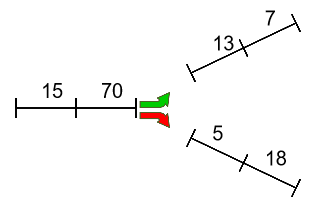
\includegraphics[width=10cm]{images/env_11_case_0}
	\label{fig:env_11_case_0}
\end{figure}\noindent
\begin{itemize}
	\item Zatory są na odcinkach 0,1,2 i 5 (odpowiednio ilości pojazdów 15,70,13,18). 
	\item Obecna faza świetlna to 0.
\end{itemize}
Prześledźmy rozwój sieci dróg. W tym celu ustalone zostaną macierze $ \textbf{S} $ oraz $ \textbf{A} $ dla powyższej sytuacji.
\def \ScaseZero {\begin{bmatrix}
		1 & 0 & 0 & 0 & 0 & 0 \\
		1 & 1 & 0 & 0 & 0 & 0 \\
		0 & 1 & 1 & 0 & 0 & 0 \\
		0 & 0 & 1 & 1 & 0 & 0 \\
		0 & 0 & 0 & 0 & 1 & 0 \\
		0 & 0 & 0 & 0 & 1 & 1 
\end{bmatrix}}
\def \AcaseZero {\begin{bmatrix}
		\frac{5}{15}  & 0             & 0             & 0 & 0 & 0 \\
		\frac{10}{15} & \frac{60}{70} & 0             & 0 & 0 & 0 \\
		0          	  & \frac{10}{70} & \frac{3}{13}  & 0 & 0 & 0 \\
		0             & 0             & \frac{10}{13} & 0 & 0 & 0 \\
		0             & 0             & 0             & 0 & 0 & 0 \\
		0             & 0             & 0             & 0 & 1 & 0 
\end{bmatrix}}

\[\textbf{S}= \ScaseZero \addtag \]
Macierz A jest następująca:
\[\textbf{A}= \AenvXI = \AcaseZero \addtag \]
\def \utMinusI{\begin{bmatrix} 
7 \\ 0 \\ 0 \\ 0 \\ 0 \\ 0 
\end{bmatrix}}
\def \xtMinusI{\begin{bmatrix} 
15 \\ 70 \\ 13 \\ 7 \\ 5 \\ 18	
\end{bmatrix}}
\def \xt{\begin{bmatrix} 
		12 \\ 70 \\ 13 \\ 10 \\ 0 \\ 5	
\end{bmatrix}} \noindent
Dla przykładu szczegółowo zostaną policzone wartości zerowej kolumny macierzy $\textbf{A}$, która dotyczy pojazdów wyjeżdżających z odcinka 0. Pozostałe wartości są liczone analogicznie.
\begin{itemize}
	\item Korzystając ze wzoru \ref{eq:manewr_zator} ustalone zostaje $f(0,1)=\frac{10}{15}$. Jest to przypadek zatoru i jedynie 10 pojazdów z 15 przemieszcza się do następnego odcinka.
	\item Wartości $f(0,2),(0,3),(0,4),(0,5)$ są równe $0$, gdyż są to przypadki \ref{eq:manewr_impossible} nieistniejących manewrów.
	\item $A[0,0]=1-\delta(0)=1-f(0,1)-f(0,2)-f(0,3)-f(0,4)-f(0,5)=1- \frac{10}{15} -0-0-0-0= \frac{5}{15}$
\end{itemize}
Ustalone zostaje, że do odcinka 0 wjeżdża z poza układu 7 pojazdów co jest przedstawione w wektorze $\textbf{u[t-1]}$. Stan w momencie $t$ wyliczony z równania stanu jest następujący:
\[\textbf{x[t]}=\textbf{A[t-1]x[t-1]}+\textbf{u[t-1]}=\AcaseZero \cdot \xtMinusI + \utMinusI = \xt \]
Poniższy obraz przedstawia sytuację w środowisku w chwili t-1 oraz przepływ pojazdów, który miał miejsce między momentem $t-1$ a $t$.
\begin{figure}[H]
	\centering
	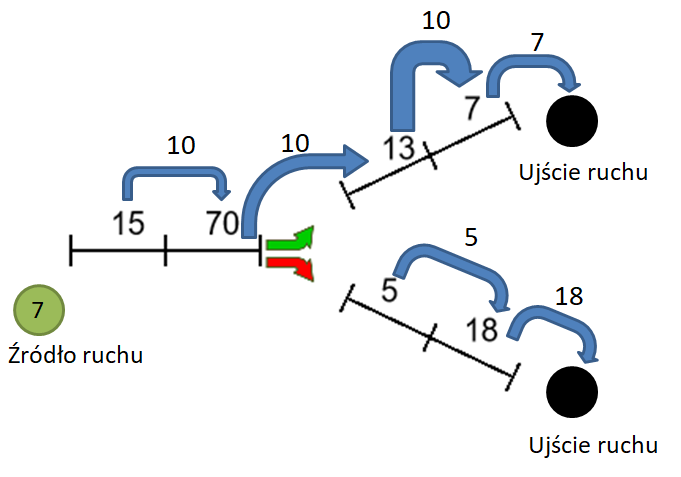
\includegraphics[width=10cm]{images/env_11_case_0_przeplyw}
	\label{fig:env_11_case_0_przeplyw}
\end{figure}\noindent
W rezultacie w chwili t obecny jest następujący stan:
\begin{figure}[H]
	\centering
	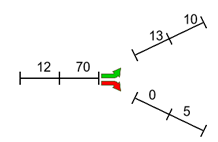
\includegraphics[width=10cm]{images/env_11_case_0_po_przeplyw_ie}
	\label{fig:env_11_case_0_po_przeplywie}
\end{figure}\noindent



\end{document} 













